\section{Проектирование программного средства}

Исходя из требований и современных стандартов разработки программное средство должно обладать следующими свойствами:
\begin{itemize}
    \item модульность;
    \item простота горизонтального масштабирования;
    \item параллельная обработка данных;
    \item безопасность хранения конфиденциальных и личных данных.
\end{itemize}

Для соответствия выше описанным свойствам было принято решение разрабатывать программное средство в виде изолированных модулей и использование архитектуры микросервисов. Так как использование монолитной архитектуры затруднит горизонтальное масштабирование и увеличит связность модулей, что усложнит последующее сопровождение. 

Разработанное программное средство состоит из следующих модулей, рисунок~\ref{fig:architecture:deployment}:
\begin{itemize}
    \item модуль выделения признаков почерка;
    \item модуль определения параметров личности;
    \item модуль контроля доступа;
    \item модуль управление образцами почерка;
    \item модуль доступа к базе данных.
\end{itemize}

Вышеописанные модули опираются на следующие группы классов, разработанные в рамках дипломного проекта:
\begin{itemize}
    \item набор классов для сегментации изображения на строки, слова, символы и выделения признаков. Написан на языке Scala с использование сторонней библиотеки Tesseract;
    \item набор классов машинного обучения (для классификации признаков текста). Написан на языке программирования Scala и содержит реализацию алгоритма основанного на методе опорных векторов (Support Vector Machine), подробнее рассмотрен в главе~\ref{sec:architecture:personal_parameters};
    \item набор классов для контроля доступа. Написана на языке Scala. Содержит классы для регистрации, авторизации и управлением сессией пользователя. Основан на стандарте JSON Web Token (JWT);
    \item набор классов для организации доступа и хранения авторизационных данным пользователя и коллекции обработанных изображений.
\end{itemize}

Далее приведено подробное описание структуры и назначения каждого модуля.

\afterpage{
  \begin{landscape}
  \thispagestyle{lscape}
  \begin{figure}[t!]
  \centering
    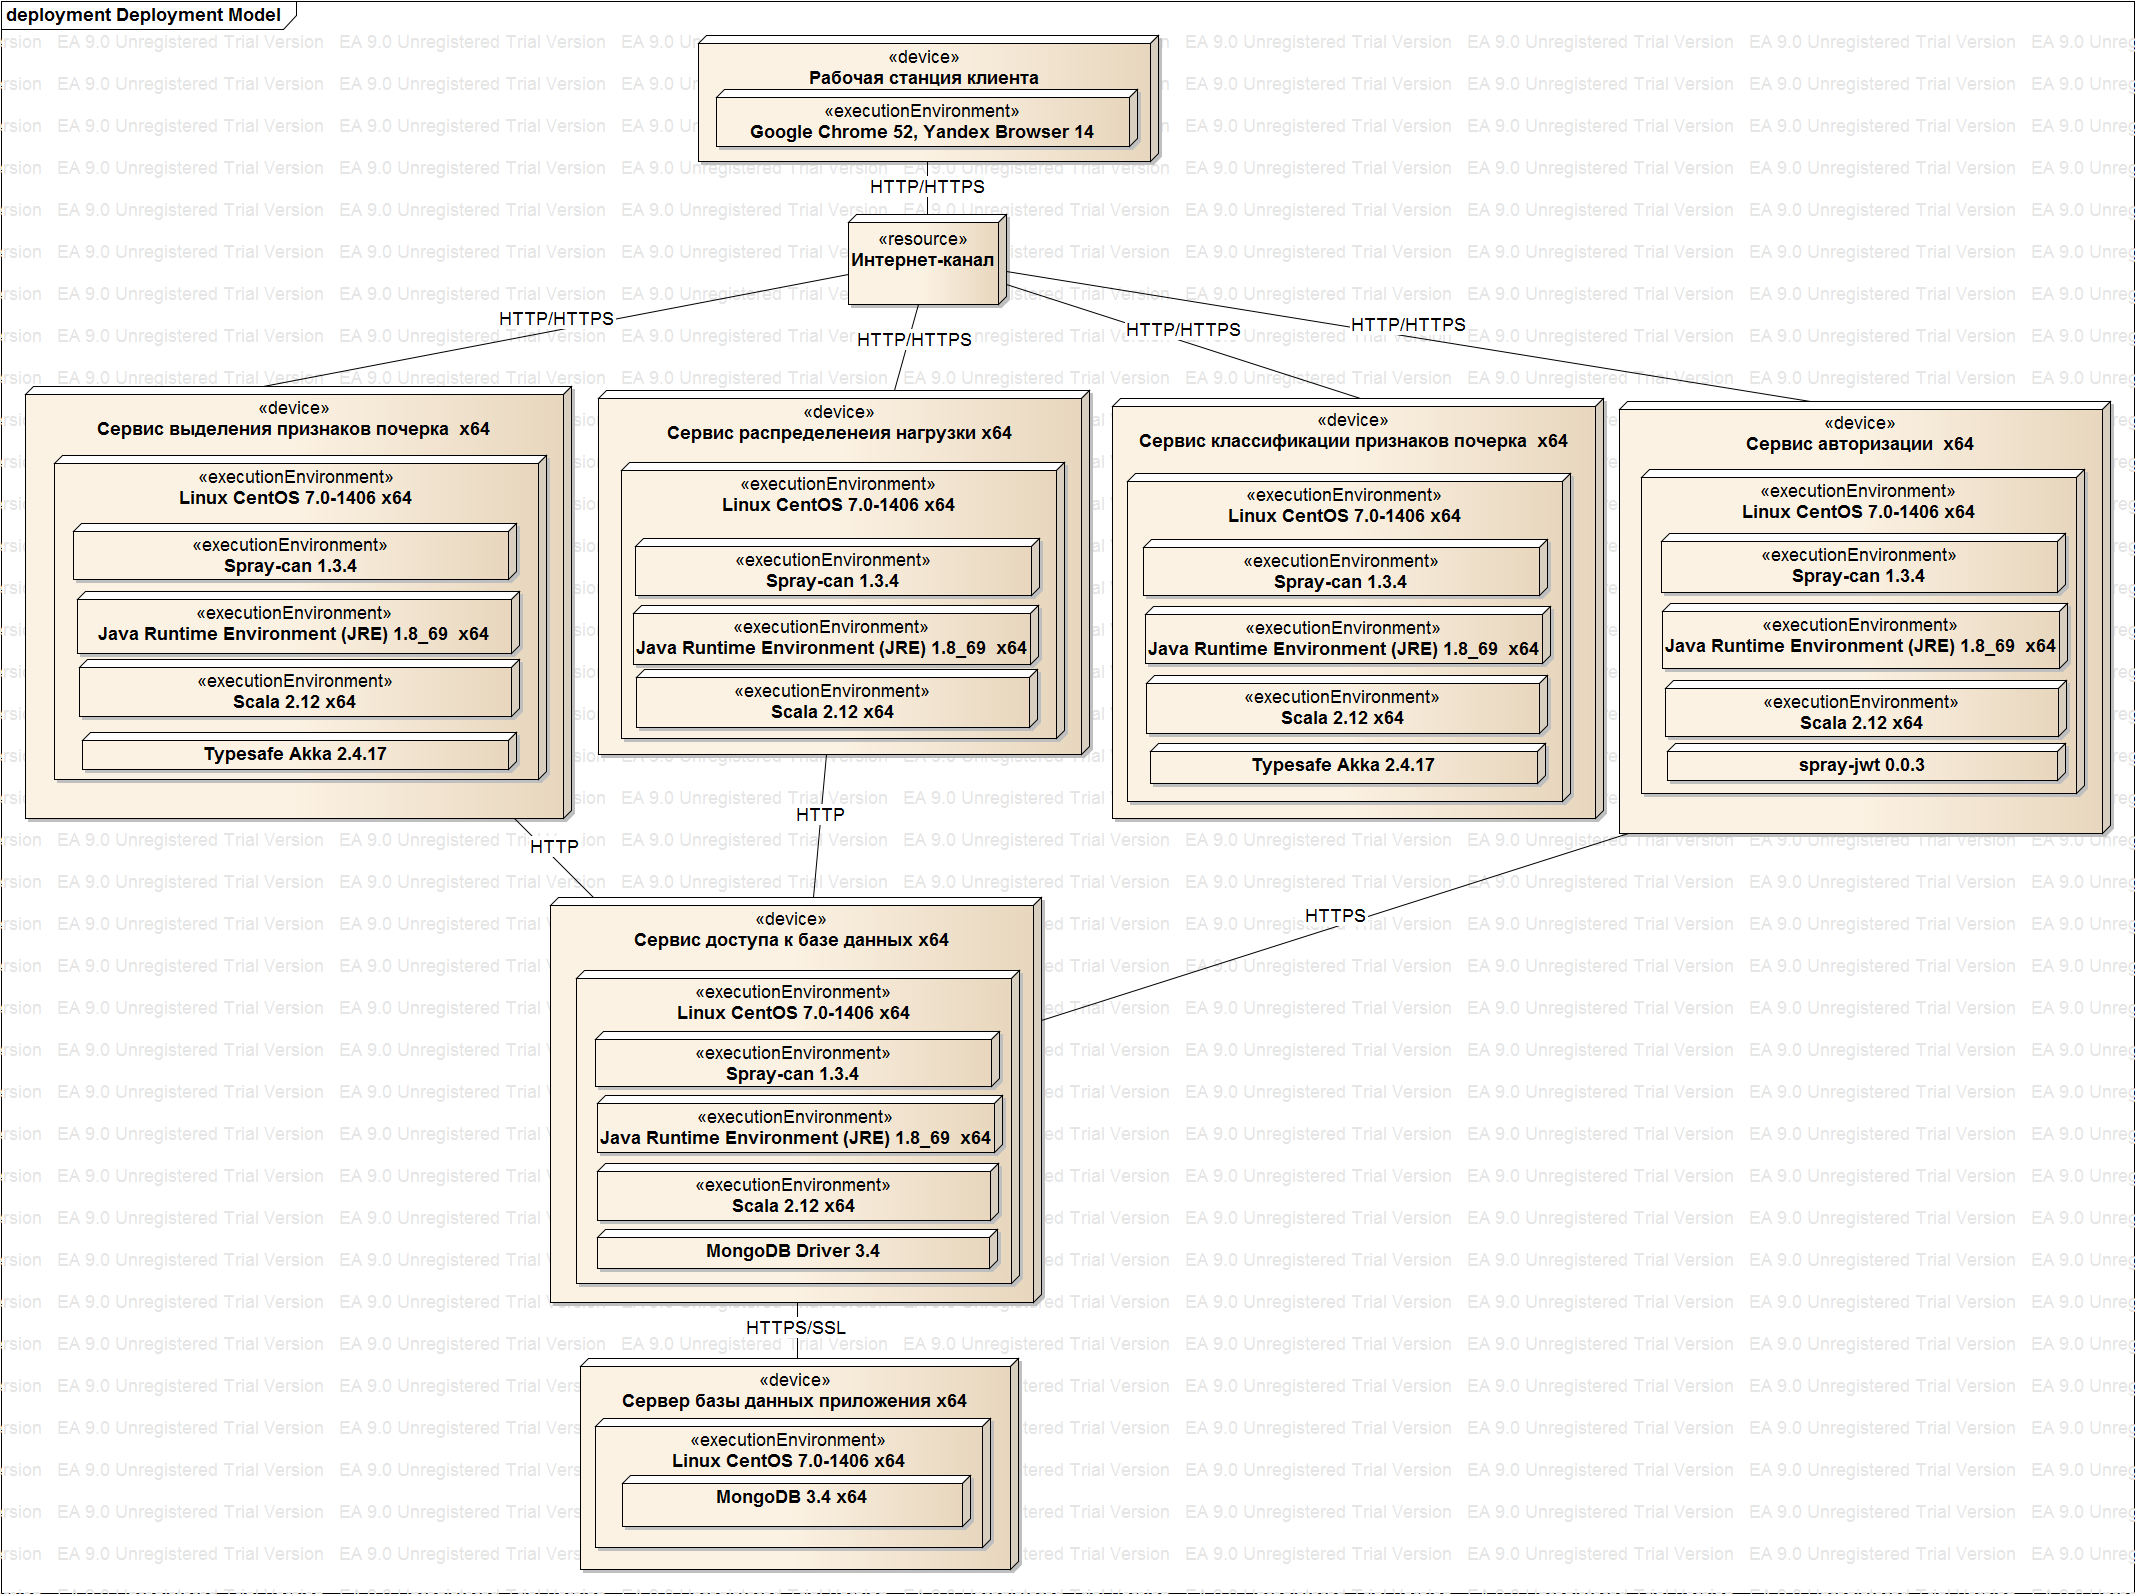
\includegraphics[scale=0.29]{figures/deployment_model.png}
    \caption{Диаграмма развертывания программного средства}
    \label{fig:architecture:deployment}
  \end{figure}
  \end{landscape}
}

\subsection{Модуль определения параметров личности}
\label{sec:architecture:personal_parameters}
Основываясь на анализе литературных источников в разделе~\ref{sub:domain:literary_sources} и спецификации требований, раздел~\ref{sec:freq:psiho_analysis}, было принято решение для определения параметров личности по признаком рукописного текста использовать классификатор на основе метода опорных векторов, широко используемого метода машинного обучения~\cite{manning_ir}, который при своей относительной простоте реализации, позволяет добиться очень неплохих результатов классификации.

Метод опорных векторов (\emph{SVM, support vector machine}) – семейство схожих алгоритмов обучения с учителем, использующихся для задач классификации и регрессионного анализа. Особым свойством метода опорных векторов является непрерывное уменьшение эмпирической ошибки классификации и увеличение зазора, поэтому метод также известен как метод классификатора с максимальным зазором~\cite{mitchell_ml, wiki_SVM}.

Параметры текста представляют собой непрерывные величины подчиняющиеся нормальному распределению, рисунок~\ref{fig:architecture:normal_pd}. Исходя их этого свойства использование полиномиальных однородных и неоднородных ядер не позволит достичь хороший результатов классификации, для достижения хороших результатов распознавания следует использовать в качестве ядер радиально-базисная функцию Гаусса~\cite{gauss_wiki}, формула~\ref{eq:architecture:gaussian_core}. 

\begin{equation}
  \label{eq:architecture:gaussian_core}
  k(x, x^{'}) = \exp(-\frac{\left|\left| x - x^{'} \right|\right|}{2\sigma_{}^2})
\end{equation}
\begin{explanation}
где & $x^{'}$ & среднее значение параметра, рассчитанное для объектов, принадлежащих
классу $C$; \\
    & $ \sigma_{}^2 $ & дисперсия значения параметра объектов из класс $C$.
\end{explanation}

Дисперсия значения параметра представлена формулой~\ref{eq:architecture:dispersion}.
\begin{equation}
  \label{eq:architecture:dispersion}
  \sigma_{}^2 = \frac{1}{n - 1} \sum\limits_{x \in C} (x_i - \overline{x_{}}^2)
\end{equation}

\begin{figure}[!h]
    \centering
    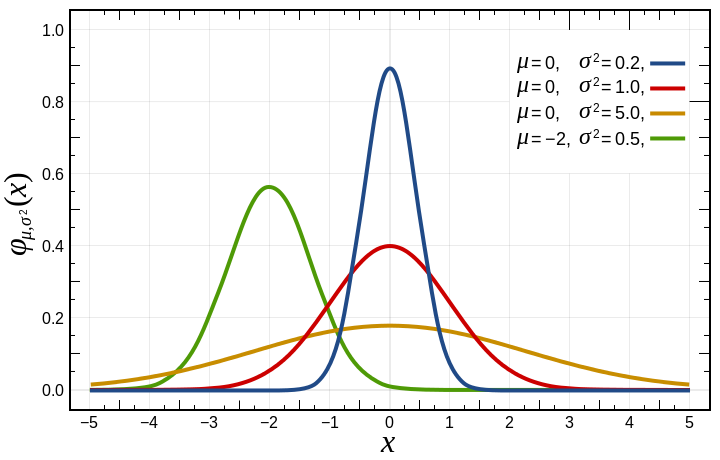
\includegraphics[width=0.85\textwidth]{figures/gauss.png}
    \caption{График функции плотности вероятности для нормального распределения}
    \label{fig:architecture:normal_pd}
\end{figure}

\subsection{Модуль выделения признаков почерка}
На основании требование сформированных в разделе~\ref{sec:freq:extract_features} основным функциями данного модуля является:
\begin{itemize}
  \item подготовка изображения к обработке (бинаризация, удаление шумов);
  \item сегментация текста (строки, слова, символы);
  \item выделения признаков почерка.
\end{itemize}

На это этапе обработки используется алгоритм линейной бинаризации по пороговому значению доминантного цвета, поскольку обработке подвергается образцы почерка с высокой вероятностью это будет цвет чернил.
Математическое выражение линейной бинаризации описывается формулой~\ref{eq:architecture:liner_binarisation}.

\begin{equation}
  \label{eq:architecture:liner_binarisation}
 \left \{
  \begin{tabular}{l}
   x <  T, x = 0 \\
   x $ \geq $ T, x = 255
  \end{tabular}
   \right .
\end{equation}
\begin{explanation}
где & $ x $ & значения яркости цвета пикселя; \\
    & Т & порог бинаризации.
\end{explanation}

Для удаления шумов используется фильтр максимума - минимума. Алгоритм работы данного фильтра основан на замене текущего пикселя на пиксель с максимальной яркостью из его окрестности при первом проходе и на пиксель с минимальной при повторном. Данный алгоритм хорошо справляется с импульсными шумами и шумами типа <<соль и перец>>.

Следующий этапам является сегментация изображения, а первой стадией сегментации является сегментация строк. 
Задача выделения строк сводиться к нахождению верхних и нижних граней строк текста на исходном изображении. Алгоритм сегментации строк основывается на том, что средняя яркость в изображениях межстрочных промежутках существенно ниже средней яркости в изображениях текстовых строк~\cite{cv_text_image_segmentator}.

Первым этапом необходимо для всех строк пикселей исходного изображения находим их средние значения яркости, формула~\ref{eq:architecture:line_medium_brigth}.
\begin{equation}
  \label{eq:architecture:line_medium_brigth}
  s_j = s_j(B) = \frac{1}{n}\cdot\sum\limits_{i=1}^{n} b_{ij}
\end{equation}

Затем необходимо определяем среднюю яркость изображения, формула~\ref{eq:architecture:medium_brigth}.
\begin{equation}
  \label{eq:architecture:medium_brigth}
  s(B) = \frac{1}{m}\cdot\sum\limits_{j=1}^{m} s_j(B)
\end{equation}

Средняя яркость в межстрочных интервалах невелика (после бинаризации близка к нулю). Поэтому яркость верхней границы можно выразить из яркости изображения, формула~\ref{eq:architecture:line_up_interval_medium_brigth}.
\begin{equation}
  \label{eq:architecture:line_up_interval_medium_brigth}
  s^{t} = k_{t} * s(B)
\end{equation}
\begin{explanation}
где & $ k_{t} $ & коэффициент от 0 до 1
\end{explanation}

Аналогично яркость нижней границы может быть выражена через яркость всего изображения, формула~\ref{eq:architecture:line_down_interval_medium_brigth}.
\begin{equation}
  \label{eq:architecture:line_down_interval_medium_brigth}
  s^{b} = k_{b} * s(B)
\end{equation}
\begin{explanation}
где & $ k_{b} $ & коэффициент от 0 до 1
\end{explanation}

Работа алгоритма заключается в последовательном просмотре массива средних значений $ (s_1,...,s_m) $ и выявлении множества пар индексов $ (s^t_i,s^b_i) $ строк пикселей соответствующих ниже приведенным условиям и следовательно являющимися верхней $ s^t_i $ и нижней $ s^b_i $ границам строк. 

Условия верхней границы текстовой строки:
\begin{itemize}
  \item яркость текущей строки пикселей превышает границу $ s^{t} $;
  \item яркость двух предыдущих строк пикселей ниже этой границы;
  \item яркость трех последующих строк выше границы $ s^{b} $.
\end{itemize}

Следовательно должно выполняться логическое условие описанное формулой~\ref{eq:architecture:logic_up_interval}.
\begin{equation}
  \label{eq:architecture:logic_up_interval}
  (s_{i-2} < s^{t}) \wedge (s_{i-1} < s^{t}) \wedge (s_i > s^{b}) \wedge (s_{i+1} > s^{b}) \wedge (s_{i+2} > s^{b}) \wedge (s_{i+3} > s^{b})
\end{equation}

Условия нижней границы текстовой строки.
\begin{itemize}     
  \item было зафиксировано начало области;
  \item яркость текущей строки пикселей превышает границу $ s^{t} $;
  \item яркость последующей строки пикселей ниже границы $ s^{b} $.
\end{itemize}
     
или

\begin{itemize}
   \item было зафиксировано начало области;
   \item яркость трех последующих строк ниже границы $ s^{b} $.
\end{itemize}

Следовательно должно выполняться логическое условие описанное формулой~\ref{eq:architecture:logic_down_interval}.
\begin{equation}
  \label{eq:architecture:logic_down_interval}
  ((s_{i+1} < s^{b}) \wedge (s_{i+2} < s^{b}) \wedge (s_{i+3} < s^{b}) \vee ((s_i > s^{t}) \wedge (s_{i+1} < s^{b})))
\end{equation}

Результатом работы алгоритма является множество пар индексов верхних и нижних границ строк. На основе этих данных можно рассчитать высоты строки (разность между индексами). Недостатком данного алгоритма является <<срезание>> символов, которые имеют высоту выше средней.

Для устранения этого недостатка можно использовать следующий прием расширения найденной границы. Необходимо определить строку с минимальной высотой $ H_{min} $, а затем границы всех строк на величину 0.3 * $ H_{min} $. Данный шаг не приведет к слиянию строк, т.к. межстрочные интервалы текста, как правило, больше чем высота строки.
 
Алгоритмы сегментации слов и символом сходи с алгоритмом сегментации строк. Основными отличиями являются необходимость построения карты яркости столбцов, а не строк, а так наличие дополнительных этапов обработки. Такими этапами являются применении <<размазывающего>> фильтра при сегментации слов и удаление ложных границ после сегментации символов.

Так же для сегментации изображения можно использовать готовый алгоритм реализованный в сторонней системы распознавания рукописного текста, например Tesseract или ABBYY FineReader. Однако данный подход требует дополнительных усилий по предварительной обработке образца почерка и лишает разработчика возможности оптимизировать алгоритм под конкретную задачу. Помимо часть подобных средств распространяеться на платной основе, что увеличит стоимость разработки и сопровождения.

Следующей функцией данного модуля является выделение из изображения признаков текста:
\begin{itemize}
  \item наклон символов;
  \item наклон строк;
  \item интервал между символами;
  \item интервал между строками;
  \item частота текста;
  \item сила нажима.
\end{itemize}

Для определения угла наклона символа необходимо определить координаты верхней и нижней точек символа и используя арктангенс вычислить угол, формула~\ref{eq:architecture:symbol_angle}.

\begin{equation}
  \label{eq:architecture:symbol_angle}
  \Theta = \tan^{-1}{\frac{y_2 - y_1}{x_2 - x_1}}
\end{equation}
\begin{explanation}
где & $\Theta$ & угол наклона символа \\
    & $ (x_1, y_1) (x_2, y_2) $ & координаты крайних точек символа.
\end{explanation}

\begin{figure}[ht]
    \centering
    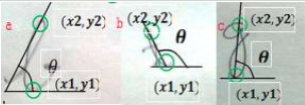
\includegraphics[width=0.85\textwidth]{figures/char_angle.png}
    \caption{Пример расчета угла наклона символа}
    \label{fig:architecture:symbol_angle}
\end{figure}

На изображении~\ref{fig:architecture:symbol_angle} приведены примеры символов с выделенными верхними и нижними точками, координаты $ (x_2, y_2) и (x_1, y_1) $ соответственно и условно обозначенным угол $ \Theta $. Представлены образцы трех типов наклона символов левосторонний, правосторонний и прямой.

Сегментация рукописного текста является нетривиальной задачей ввиду непостоянства таких параметров как пробелы между символами, в плодь до их отсутствия, словами и строками. Задача становится еще сложнее учитывая то, что данные признаки необходимо сохранить и использовать в дальнейшей работе. Так же стоит отметить что выделения силы нажатия необходимо производить до бинаризации, т.к. после бинаризации это будет невозможно.

Поскольку сегментации изображения и выделение признаков являются относительно долгими операциями, сегментация вместе с выделением признаков занимает от 0.5 до 3 секунд, в зависимости от размера изображения, обеспечение параллельной обработки выходит на передний план. К счастью выбранные признаки почерка независимы и могут рассчитываться параллельно. Так же нет необходимость ожидать полной сегментации изображения для начала выделения признаков, например интервал между строками можно вычислить сразу после разбиения изображения на строки. Это позволит значительно ускорить работу данного модуля.

\subsection{Модуль контроля доступа}
Поскольку разрабатываемое приложение может содержать персональные данные пользователя, вплоть до имени и фамилии в графе комментариев к изображению, задача организации безопасного доступа и хранению подобных данных стоит довольно остро.
Данный модуль отвечает за регистрацию и авторизацию пользователей. 
В данном проекте для предоставления защищенного доступа к модулям будет использоваться открытый стандарт JSON Web Token (RFC 7519). JWT-маркер  содержит в зашифрованном виде всю минимально необходимую информацию для аутентификации и авторизации. При этом не требуется хранить в сессии данных о пользователе, так как маркер самодостаточный. Данный факт упрощает горизонтальное масштабирование системы и хорошо подход для архитектур на основе микросервисов.

На основании требование сформированных в разделах~\ref{sec:freq:reg} и~\ref{sec:freq:auth} и основными функциями данного модуля являются:
\begin{itemize}
  \item регистрации новых пользователей;
  \item авторизация пользователей;
  \item генерация JWT маркеров.
\end{itemize}

Обобщенный алгоритм генерации и верификации JWT-маркеров:
\begin{figure}[ht]
    \centering
    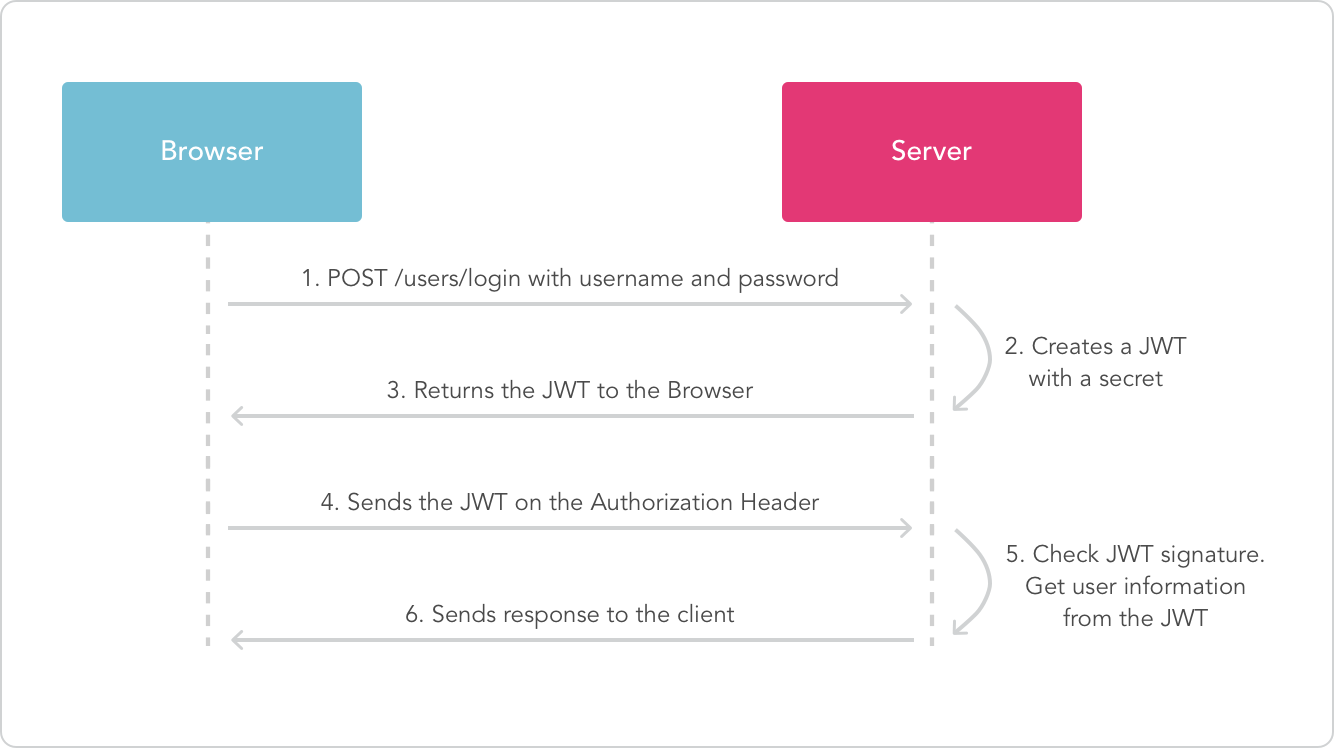
\includegraphics[width=0.7\textwidth]{figures/jwt_diagram.png}
    \caption{Диаграмма генерации и верификации JWT-маркеров}
    \label{fig:architecture:jwt_diagram}
\end{figure}

На рисунке~\ref{fig:architecture:jwt_diagram} представлен алгоритм создания, подписи и проверки JWT-маркера. В данном примере выдачу и проверку маркера осуществляет один и тот же сервер, однако, как было описано выше, это не является обязательным условием и представлено лишь для упрощения диаграммы.

Использование контроля доступа на основе JWT-маркеров позволяет снизить нагрузку на сервис контроля доступа, благодаря возможности проверки подлинности маркета на стороне других сервисов, а так же не накладывает существенных ограничений на количество и географическое расположение сервисов системы.

\subsection{Модуль доступа к данным}
Данный модуль отвечает за организацию работы в базой данных и предоставление другим модулям удобного интерфейса.
На основании требование сформированных в разделах~\ref{sec:freq:show},~\ref{sec:freq:add},~\ref{sec:freq:delete} и~\ref{sec:freq:package_add} основными функциями данного модуля являются:
\begin{itemize}
  \item добавление авторизационных данных пользователя в базу при регистрации (включая проверку дублирования имен пользователей);
  \item проверка наличия пользователя в базе и соответствие хеша пароля;
  \item добавление нового изображения в базу;
  \item обновление информации о параметрах изображения;
  \item удаление изображения из базы.
\end{itemize}

Так как список параметров изображения не постоянный и параметры рассчитываются и обновляются параллельно, использование классической реляционной базы данных в данном случае нерационально, в тоже время на базу данных на налагается каких-либо существенных ограничений по быстродействию и скорости обработки запросов. Основываясь на выше перечисленном в качестве СУБД была выбрана MongoDB
Так же плюсом этого решения можно отнести хранение документов в базе в виде JSON-объектов, что исключает дополнительное преобразование данных перед отправкой их другим сервисам и на клиент, а так же отсутствие платы за использование, что позволит снизить стоимость разработки и использования.